% Asset ID: AS1AlgebraicMethodsTikZ-001
% Unit code: AS1
% Topic code: AS1-AF
% Topic ID: AS1AlgebraicMethodsFactorTheorem
% Related LO IDs: AS1-AF-LO010, AS1-AF-LO011
% Source: CCEA Mathematics Specification Map; Chapter 7a Algebraic Methods transcript; Dr Frost Algebraic Methods PDF
% Related lesson section: Core Theory B-E: Polynomial Long Division by Linear Expressions
% Purpose: Provide a clean printable TikZ diagram for polynomial long division by a linear expression.

\documentclass[tikz,border=8pt]{standalone}
\usepackage{amsmath}
\usepackage{amssymb}
\usetikzlibrary{arrows.meta, positioning, calc, decorations.pathreplacing}
\begin{document}
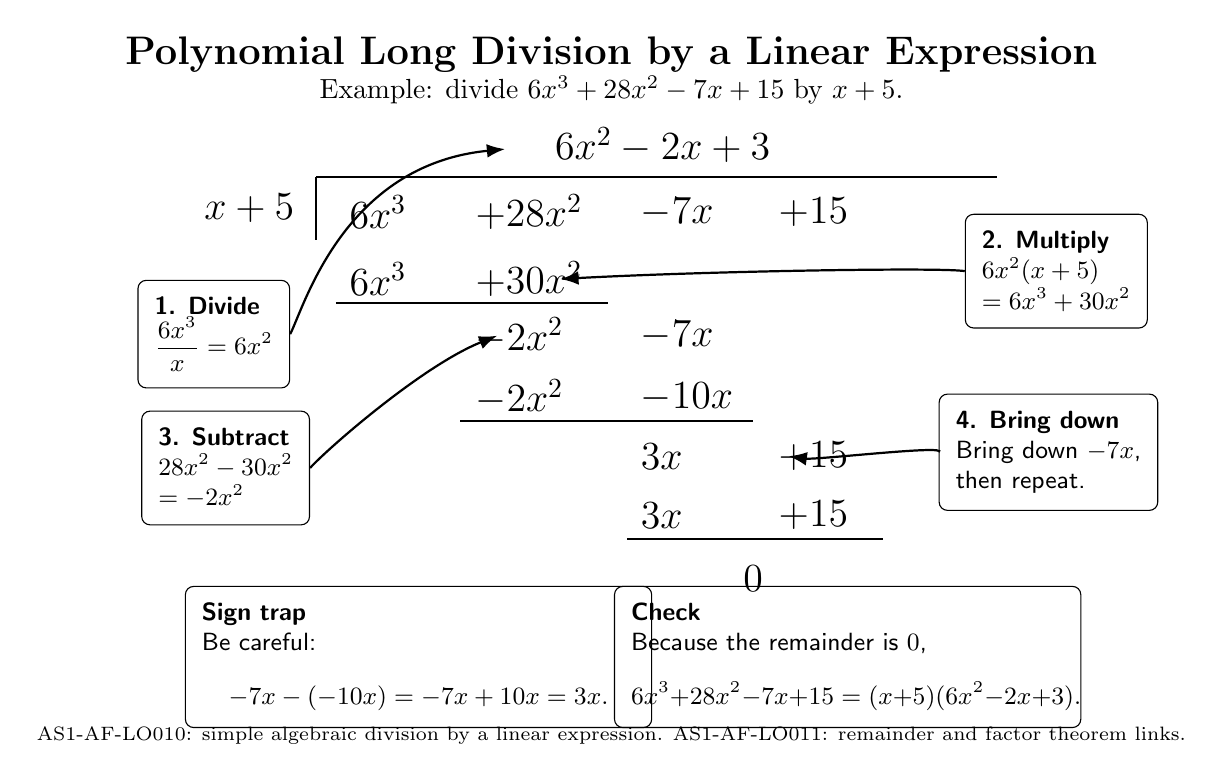
\begin{tikzpicture}[
    every node/.style={font=\sffamily},
    mathnode/.style={font=\Large},
    smallmath/.style={font=\normalsize},
    labelbox/.style={draw,rounded corners=3pt,align=left,inner sep=6pt,font=\small\sffamily},
    arrow/.style={-Latex, thick}
]
\node[font=\bfseries\Large] at (6,8.2) {Polynomial Long Division by a Linear Expression};
\node[font=\normalsize] at (6,7.75) {Example: divide \(6x^3+28x^2-7x+15\) by \(x+5\).};
\node[mathnode] (divisor) at (1.4,6.25) {\(x+5\)};
\draw[thick] (2.25,6.65) -- (2.25,5.85);
\draw[thick] (2.25,6.65) -- (10.9,6.65);
\node[mathnode] at (6.65,7.05) {\(6x^2-2x+3\)};
\node[mathnode, anchor=west] at (2.55,6.20) {\(6x^3\)};
\node[mathnode, anchor=west] at (4.15,6.20) {\(+28x^2\)};
\node[mathnode, anchor=west] at (6.25,6.20) {\(-7x\)};
\node[mathnode, anchor=west] at (8.00,6.20) {\(+15\)};
\node[mathnode, anchor=west] at (2.55,5.35) {\(6x^3\)};
\node[mathnode, anchor=west] at (4.15,5.35) {\(+30x^2\)};
\draw[thick] (2.50,5.05) -- (5.95,5.05);
\node[mathnode, anchor=west] at (4.15,4.63) {\(-2x^2\)};
\node[mathnode, anchor=west] at (6.25,4.63) {\(-7x\)};
\node[mathnode, anchor=west] at (4.15,3.85) {\(-2x^2\)};
\node[mathnode, anchor=west] at (6.25,3.85) {\(-10x\)};
\draw[thick] (4.08,3.55) -- (7.80,3.55);
\node[mathnode, anchor=west] at (6.25,3.10) {\(3x\)};
\node[mathnode, anchor=west] at (8.00,3.10) {\(+15\)};
\node[mathnode, anchor=west] at (6.25,2.35) {\(3x\)};
\node[mathnode, anchor=west] at (8.00,2.35) {\(+15\)};
\draw[thick] (6.20,2.05) -- (9.45,2.05);
\node[mathnode] at (7.80,1.55) {\(0\)};
\node[labelbox] (step1) at (0.95,4.65) {\textbf{1. Divide}\\ \(\dfrac{6x^3}{x}=6x^2\)};
\draw[arrow] (step1.east) .. controls (2.1,5.0) and (2.6,6.8) .. (4.65,7.00);
\node[labelbox] (step2) at (11.65,5.45) {\textbf{2. Multiply}\\ \(6x^2(x+5)\)\\ \(=6x^3+30x^2\)};
\draw[arrow] (step2.west) .. controls (10.2,5.5) and (7.2,5.45) .. (5.35,5.35);
\node[labelbox] (step3) at (1.1,2.95) {\textbf{3. Subtract}\\ \(28x^2-30x^2\)\\ \(=-2x^2\)};
\draw[arrow] (step3.east) .. controls (2.4,3.2) and (3.6,4.25) .. (4.55,4.63);
\node[labelbox] (step4) at (11.55,3.15) {\textbf{4. Bring down}\\ Bring down \(-7x\),\\ then repeat.};
\draw[arrow] (step4.west) .. controls (10.3,3.25) and (8.6,3.05) .. (8.25,3.10);
\node[labelbox, text width=5.5cm] at (3.55,0.55) {\textbf{Sign trap}\\ Be careful: \[-7x-(-10x)=-7x+10x=3x.\]};
\node[labelbox, text width=5.5cm] at (9.00,0.55) {\textbf{Check}\\ Because the remainder is \(0\), \[6x^3+28x^2-7x+15=(x+5)(6x^2-2x+3).\]};
\node[font=\scriptsize] at (6,-0.45) {AS1-AF-LO010: simple algebraic division by a linear expression. AS1-AF-LO011: remainder and factor theorem links.};
\end{tikzpicture}
\end{document}
